%%%%%%%%%%%%%%%%%%%%%%%%%%%%%%%%%%%%%%%%%%%%%%%%%
%
%       Chapter 1 - Introduction
%
%%%%%%%%%%%%%%%%%%%%%%%%%%%%%%%%%%%%%%%%%%%%%%%%%

\chapter{Introduction}

Statistical Machine Translation (SMT) enables translation between various languages, such as French, German, Chinese, English, etc. With the advent of Google Translate and their support for translation between 81 languages, translation services have become available to the masses for day to day use. Current state of the art SMT utilize words, sub-phrases and phrases in the parallel text (corpora containing translations of same text in two languages) to build fluent and accurate translation systems. In order to create such translation systems, machine learning methods are applied over the statistical information extracted from parallel text to develop models for translation.

Phrase-based SMT \cite{Koehn2003} uses contiguous sequence of words (phrases) as the unit of translation. In this, each source phrase is translated to a non-empty target phrase, where the source and target phrases can be of different lengths. The translation process of phrase-based SMT can be divided into three steps, as described in the survey by Adam Lopez \cite{Lopez2008}:
\begin{enumerate}
\item Split the sentence into phrases.
\item Translate each phrase
\item Permute over each translated phrase to get the final order.
\end{enumerate}

When translating each source phrase to the target language, the SMT system only has information of source words in the current source phrase. Information from source words outside the current source phrase is incorporated only indirectly, via target words that are translations of these source words, if the relevant target words are close enough to the current target word to affect the language model probability scores. SMT systems use language models to determine how fluent is the translation. To add more information about source outside the current source phrase \cite{Niehues2011} introduced bilingual language models that use alignments between source words and target words to create bitokens. A language model was then estimated using the bitokens. When using bitokens, the vocabulary expands significantly. To counter this, \cite{Niehues2011} replaced words in the corpus with their part-of-speech tags and then created the bitokens. \cite{Stewart2014} extended this work by clustering the words in the original corpus using a Brown clustering algorithm. They also clustered the bitokens before estimating the bilingual language models. 

But, in these approaches, bilingual information is available only through word alignments. And, state of the art word alignment algorithms have a high error rate. In order to compensate for the alignment errors and to add more information from source words which are not only direct translations of target words but are also semantically similar to the target words, we introduce a new approach to train bilingual language models using monolingual and bilingual word embeddings.

In the next section we give an introduction to statistical machine translation and the steps involved in building an SMT system.

\section{Statistical Machine Translation}
The process of building a phrase-based SMT system using a parallel corpus can be broadly divided into five modules:
\begin{enumerate}
	\item Learn bi-directional alignments of words.
	\item Extract phrase pairs from the alignments and calculate probability of each translation pair, called the \textit{translation model}.
	\item Estimate language models.
	\item Tune the parameters for features used in the system.
	\item Using the \textit{language model} and \textit{translation model}, decode the translation of a new source language sentence into target language sentence.
\end{enumerate}

In this thesis, we focus on \textit{Module 3 and 5}, that are, estimating language models and using language models while decoding a new source language sentence. In the next sub-sections, we give a brief overview on each of the modules in an SMT system.

\subsection{Word Alignments}\label{section:alignments}
Word alignment is the task of identifying translation relationships between words of sentence aligned parallel corpora. By sentence aligned parallel corpora, we mean a parallel corpus in which each sentence in the source language is aligned with the same sentence in the target language. Word alignments do not have to be a one-to-one mapping. Words in one language can be aligned to more than one words or no words at all in the other language. Figure \ref{fig:sample-align} shows alignment matrix between a Spanish sentence and English sentence. As shown in the example, the English word \textit{slap} is aligned to three Spanish words \textit{daba una bofetada}.

\begin{figure}[h]
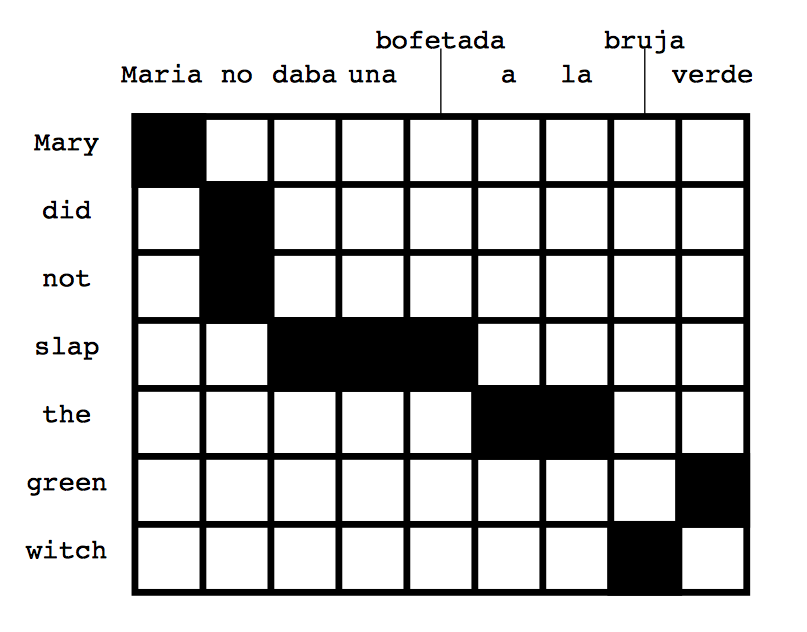
\includegraphics[width=10cm]{files/images/alignmentExample}
\centering
\caption{A sample alignment between a Spanish sentence and English sentence \cite{Koehn2009}}
\label{fig:sample-align}
\end{figure}

It is not easy to find accurate alignments between words of two languages. Specially, for some function words which may or may not have an equivalent word in the other language. Also, it is important that content words in source language are aligned to the corresponding content word in the target language.

Approaches for learning word alignments can be classified into two general categories, as described by \cite{Och2003}, \textit{(a) statistical alignment models}, and \textit{(b) heuristic models}. In this thesis we only focus on \textit{statistical alignment models} and look at various methods in this category. 

In statistical alignment models, we collect statistics from the sentence aligned parallel corpus to generate word alignment models. We are given a source language string $f^J_1 = f_1,..., f_j, ..., f_J$ and a target language string $e^I_1 = e_1, ..., e_i, ..., e_I$. In SMT, we have a translation model $P(f^J_1 | e^I_1)$, which is the translation probability describing the relationship between a source language string and target language string. In this translation model, we introduce a \textit{hidden} alignment $a^J_1$ which describes the mapping between word $f_j$ and $e_i$. This gives us the statistical alignment model as $P(f^J_1, a^J_1 | e^I_1)$. As shown by \cite{Och2003}, the relation between translation model and statistical alignment model is
\begin{eqnarray}
P(f^J_1 | e^I_1) = \sum_{a^J_1} P(f^J_1, a^J_1 | e^I_1)
\end{eqnarray}

To account for the unknown parameters $\theta$ learnt from training data, the statistical alignment model is represented as $p_{\theta}(f^J_1, a^J_1 | e^I_1)$. For each sentence pair $(\mathbf{f_n, e_n})$, for $n = 1, ..., N$, where $N$ is the size of parallel corpus, the alignment is denoted as $\mathbf{a} = a^J_1$. We find the unknown parameters $\theta$ by maximizing the likelihood on the parallel corpus:

\begin{eqnarray}
\hat{\theta} = \arg\!\max_\theta \prod_{n = 1}^{N} \sum_{\mathbf{a}} p_{\theta}(\mathbf{f_n}, \mathbf{a} | \mathbf{e_n})
\end{eqnarray}

To perform the maximization, Expectation Maximization (EM) \cite{Dempster1977} or some variant of it is used. After finding the unknown parameters, the best alignment for a pair of sentences can be calculated as:

\begin{eqnarray}
\hat{a}^J_1 = \arg\!\max_{a^J_1} p_{\hat{\theta}}(f^J_1, a^J_1 | e^I_1)
\end{eqnarray}

Such statistical alignment models are called generative models and are generally created using unsupervised learning techniques. A major drawback of generative models is that incorporating arbitrary features is difficult. For example, if we want to include orthographic similarity between two words, presence of the pair in some dictionary, etc. Another drawback of unsupervised generative models based on EM is that they require large amount of data and processing to converge to a good solution. Discriminative models on the other hand allow us to have arbitrary features. In discriminative models the features do not have to adhere to the independence assumption, that is, features can be dependent on other features. Whereas, generally in generative EM based algorithms, we assume that the features are independent of each other. 

There are various ways to create discriminative models for getting word alignments. Word alignment problem can also be thought of as a maximum weighted matching problem where each pair of words in parallel sentences would be assigned a score depending on how likely they are to be aligned. The word alignment problem can also be considered as a maximum weight bipartite matching problem \cite{Taskar2005}, where nodes correspond to words in the two parallel sentences. Aside from graph matching algorithms, discriminative approaches also use perceptron algorithm \cite{Moore2006}, support vector machines \cite{Cherry2006}, conditional random fields \cite{Blunsom2006} or neural networks \cite{Ayan2005}.

%Apart from the unsupervised learning approach, statistical alignment models can also be created using semi-supervised or supervised learning. In both these techniques, manually annotated alignments of words in parallel sentences are utilized to train the model. In supervised training, the complete training parallel corpus would be manually annotated. In semi-supervised training, only few examples from the complete training corpus are manually annotated and used for training the models. Both these approaches use a held out set of manual alignments to tune the model parameters.
%Even though, supervised learning would allow us to achieve better performance of the model, but getting manually annotated parallel corpus for training is expensive. Semi-supervised learning allows us to reach convergence of the optimization function at a faster rate as compared to unsupervised technique by only using small amount of manually annotated parallel corpus.

\subsection{Translation Model}\label{intro-tm}
In phrase-based SMT, continuous sequence of words (phrases) are the atomic units of translation. The source sentence is first broken down into phrases and each phrase is then translated. To get the translation of source phrase, a phrase table is learnt from the parallel corpora. \cite{Koehn2009} states the following advantages of using phrases as atomic units:
\begin{itemize}
	\item Many-to-many translation can handle non-compositional phrases.
	\item Use of local context in translation.
	\item Longer phrases can be learnt if more data is available.
\end{itemize}

The learning of phrase table can be broken down into three steps:
\begin{itemize}
	\item Get alignments (as described in Section~\ref{section:alignments}) of words from parallel corpora in both directions (bi-directional alignments). To combine the alignments from two runs, there are various heuristics in the literature, but for our work, we use the approach outlined in \cite{Koehn2003} called \textit{grow-diag-final-and}. This heuristic has several steps, in the first step, all \textit{intersection} alignment points are selected. In the \textit{grow-diag} step, neighbouring and diagonally neighbouring alignment points which are in the union but not in the intersection of the two runs are selected. And, in \textit{final-and} step, alignment points which are unaligned and present in the \textit{intersection} are selected . For our work, we use GIZA++ \cite{Och2003} to get the bidirectional alignments.
	
	\item Using the bidirectional alignments from step 1, extract all posible phrase pairs which are consistent with the alignments \cite{Och1999, Koehn2003}. A phrase pair is consistent with the alignments if words within the source phrase are only aligned to words in the target phrase. Table~\ref{table:sample-phrase-pairs} shows all the posible phrase pairs that are consistent with the alignments shown in Fig~\ref{fig:sample-align}.
	
	\item Assign probabilities to phrase pairs using their relative frequencies:
	\begin{eqnarray}
		\phi(\bar{f}|\bar{e}) = \frac{count(\bar{e}, \bar{f})}{\sum_{\bar{f_i}} count(\bar{e}, \bar{f_i})}
	\end{eqnarray}
	Here, $\bar{f}$ is a source phrase and $\bar{e}$ is the target phrase. Along with $\phi(\bar{f} | \bar{e})$, other features like \textit{inverse lexical weighting}, \textit{direct phrase translation probability} and \textit{direct lexical weighting} are also calculated.
\end{itemize}

\begin{table}
	\begin{center}
		\begin{tabular}{|c|c|}
			\hline
			\textbf{Source Phrase} & \textbf{Target Phrase} \\\hline
			Maria & Mary\\
			no & did not \\
			daba una bofeta & slap \\
			a la & the \\
			bruja & witch \\
			verde & green \\
			Maria no & Mary did not \\
			no daba una bofetada & did not slap \\
			daba una bofetada a la & slap the \\
			bruja verde & green witch \\
			Maria no daba una bofetada & Mary did not slap \\
			no daba una bofetada a la & did not slap the \\
			a la burja verde & the green witch \\
			Maria no daba una bofetada a la & Mary did not slap the \\
			daba una bofetada a la burja verde & slap the green witch \\
			no daba una bofetada a la burja verde & did not slap the green witch \\
			Maria no daba una bofetada a la burja verde & Mary did not slap the green witch \\ \hline
		\end{tabular}
		\caption{All possible phrase pairs consistent with the alignments shown in Fig.\ref{fig:sample-align}}
		\label{table:sample-phrase-pairs}		
	\end{center}
\end{table}

At the end of these steps, we get a phrase table containing the bilingual phrase pairs, the alignments within those phrase pairs and feature scores as shown in table~\ref{table:sample-phrase-table-entry}.

\begin{table}
	\begin{center}
		\begin{tabular}{|c|c|c|c|}
			\hline
			\textbf{Source Phrase} & \textbf{Target Phrase} & \textbf{Feature Scores} & \textbf{Alignments}\\\hline
			in europa & in europe & 0.829007 0.207955 0.801493 0.492402 & 0-0 1-1 \\\hline
		\end{tabular}
		\caption{A sample entry in the translation model (phrase table)}
		\label{table:sample-phrase-table-entry}		
	\end{center}
\end{table}


\subsection{Language Model}\label{intro-lm}
Language model is an integral part of an SMT system. The job of a language model is to measure how likely a string of words (sentence) in a language would be uttered by a human speaker, that is, how fluent is the sentence. For example, we have two sentences in English, \textit{"this is a house"} and \textit{"this a house is"}. The language model should tell us that the probability of former sentence should be higher than the latter, that is, $p_{LM}(\textnormal{\textit{this is a house}}) > p_{LM}(\textnormal{\textit{this a house is}})$. From this example, we notice that language models along with telling how fluent a sentence is, they also help in deciding the right order of words. They also help in choosing the right words for translation. For example, $p_{LM}(\textnormal{\textit{I am going home}}) > p_{LM}(\textnormal{\textit{I am going house}})$.

For an SMT system, the language model is trained on large monolingual corpora of the target language. This is because we want to aid the translation system in deciding a good translation for a source sentence. Due to abundance of data available in a single language, the amount of training data used in training the language model is generally orders of magnitude more than the parallel corpora used to train the translation model. 

The state of the art method to train a language model is \textit{n-gram} language modelling. In n-gram language models, we compute the probability of a sentence $W = w_1, w_2, w_3,..., w_n$. The probability of sentence $p(W)$ can be represented as a joint probability of words in the sentence: 
\begin{eqnarray}
	p(W) = p(w_1, w_2, ..., w_n)
\end{eqnarray}

Using chain rule, we can break this down:
\begin{eqnarray}
p(W) = p(w_1)p(w_2|w_1)p(w_3| w_1, w_2)...p(w_n|w_1, w_2, ...,w_{n-1})
\end{eqnarray}

Here, we have broken down the probability of a sentence into probability of words depending on the preceeding words. To be able to calculate these probabilities easily, we limit the history of each word to $m$ words.
\begin{eqnarray}
p(W) = p(w_1)p(w_2|w_1)p(w_3| w_1, w_2)...p(w_n|w_{n-m}, ...,w_{n-2}, w_{n-1})
\end{eqnarray}
This model in which we step through a sequence of words and consider a limited history for each transition is called a \textbf{Markov chain}. Here $m$ is the order of the model. For example, a 3 gram language model would be:
\begin{eqnarray}
p(W) = p(w_1)p(w_2|w_1)p(w_3| w_1, w_2)p(w_4|w_2, w_3)...p(w_n|w_{n-2}, w_{n-1})
\end{eqnarray}

To estimate the probability of the n-grams, we collect the required counts from the monolingual corpora and use maximum likelihood estimation:
\begin{eqnarray}
p(w_3|w_1, w_2) = \frac{count(w_1, w_2, w_3)}{\sum_{w} count(w_1, w_2, w)}
\end{eqnarray}

%Even though we use a large monolingual corpora to train the language model, we still cannot cover every word and it's usage. To tackle the problem of unseen words, the literature describes various smoothing techniques like \textit{add-one smoothing} and \textit{add-\alpha smoothing}. In add-one and add-\alpha smoothing, we add add 1 or some number \alpha > 1 to the count of each word and add the count of vocabulary or \alpha times vocabulary to the normalizer.
Even though we use a large monolingual corpora to train the language model, we still cannot cover every word and it's usage. To tackle the problem of unseen words, the literature describes various smoothing techniques like \textit{add-one smoothing}, \textit{add-$\alpha$ smoothing}, \textit{Good-Turing smoothing} \cite{Good1953}, \textit{Witten-Bell smoothing} \cite{WittenBell1991}, \textit{Kneser-Ney smoothing} \cite{KneserNey1995}, etc. 

\subsection{Decoder}\label{intro-decoder}
\cite{Koehn2003} states the mathematical model for translation as $p(e|f)$. The job of the decoder is to find the translation $e_{best}$ with the highest probability. This can be mathematically formulated as:
\begin{eqnarray}
	e_{best} = {argmax}_e p(e|f)
\end{eqnarray}

\begin{figure}[h]
	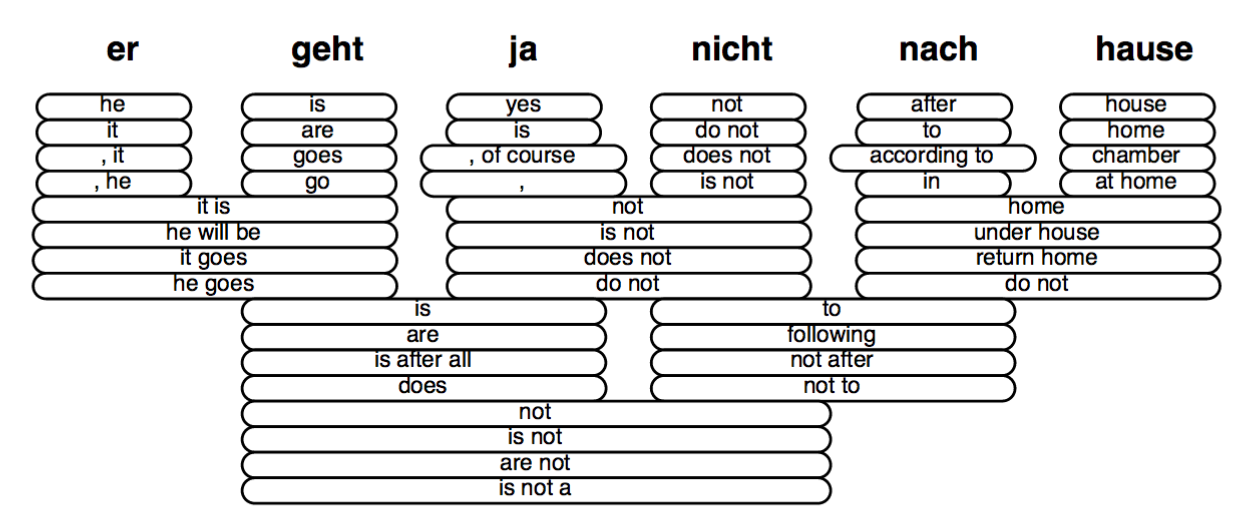
\includegraphics[width=10cm]{files/images/translation-options}
	\centering
	\caption{A sample German source sentence broken into possbile phrases and the top four translation options for each of the source phrase \cite{Koehn2009}}
	\label{fig:sample-translation-options}
\end{figure}

When the decoder proposed by \cite{Koehn2003} has to translate a source sentence, it first breaks the sentence down into the atomic units of phrase-based SMT, that is, phrases as shown in Fig~\ref{fig:sample-translation-options}. The target sentence is then generated left to right in the form of partial translations called hypothesis and it employs a beam search algorithm. The decoder starts with an initial empty hypothesis. A new hypothesis is expanded from an existing hypothesis by selecting the next untranslated source phrase, finding it's possible target phrase from the translation model. The target phrase is appended to the existing target sentence. The hypothesis is then scored using weighted combination of scores from certain feature functions and the source phrase is marked as translated. The final hypothesis in the search tree which has the highest probability is chosen as the best translation for the source sentence as shown in Fig~\ref{fig:sample-search}

\begin{figure}[h]
	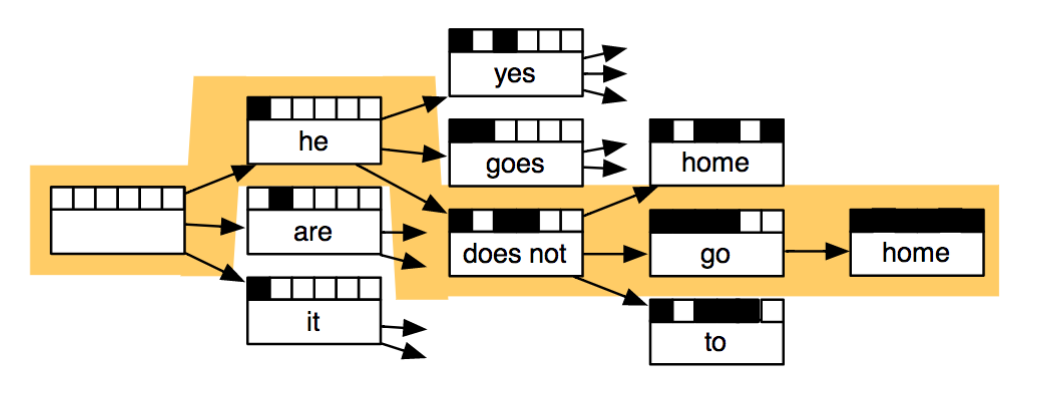
\includegraphics[width=10cm]{files/images/sample-search}
	\centering
	\caption{A sample German source sentence broken into possbile phrases and the top four translation options for each of the source phrase \cite{Koehn2009}}
	\label{fig:sample-search}
\end{figure}

A limitation of this approach is that for each source sentence, exponential number of hypothesis are generated. Searching through these hypothesis is an NP-complete problem \cite{Knight1999}. To tackle this problem, \cite{Koehn2003} proposed using the hypothesis recombination strategy as in \cite{Och2001}. Along with this, hypothesis are also pruned by comparing their current score and the future score proposed by \cite{Koehn2003}. Histogram pruning and threshold pruning proposed by \cite{Koehn2004Pharaoh} are also used to prune the search tree.

We mentioned above that the decoder scores each hypothesis using a weighted combination of scores from various feature functions. We also mentioned above that the decoder uses translation model in it's process. In addition to the feature scores from translation model, the decoder also uses the language model we described earlier, a reordering model which is created using the alignments extracted earlier and various feature functions.

\cite{Koehn2003} proposed a weighted model comprising of the phrase translation model ($\phi(\bar{f}|\bar{e})$), a reordering model ($d$), and language model ($p_{LM}(e)$), which is mathematically formulated as:
\begin{eqnarray}\label{eqn:weighted-model}
	e_{best} = {argmax}_e \prod_{i=1}^{I} \phi(\bar{f}_i|\bar{e}_i)^{\lambda_\phi} d(a_i - b_{i_1} -1)^{\lambda_d} \prod_{i=1}^{|e|}p_{LM}(\textbf{e})^{\lambda_{LM}}
\end{eqnarray}
Here $a_i$ and $b_{i_1}$ are the starting and ending position of the source phrase that was translated to the $i^{th}$ target phrase and ${i-1}^{th}$ target phrase. $\lambda_\phi$, $\lambda_d$ and $\lambda_{LM}$ are the weights for translation model, reordering model and language model respectively. These scores are calculated incrementally for each hypothesis.

Such a weighted model is actually a log-linear model of the form:
\begin{eqnarray}
	p(x) = exp \sum_{i=1}^{n}\lambda_ih_i(x)
\end{eqnarray}

When working with probabilities, it is easier to deal with log values to avoid floating point underflow problems. We can rewrite equation~\ref{eqn:weighted-model} as:
\begin{eqnarray}
	\begin{aligned}
		p(e, a|f)& = exp \big[\lambda_\phi \sum_{i=1}^{I}\log\phi(\bar{f}_i|\bar{e}_i) \\
		& + \lambda_d \sum_{i=1}^{I}\log d(a_i - b_{i-1} -1) \\
		& + \lambda_{LM} \sum_{i}^{|e|} \log p_{LM}(e_1 | e_1 ... e_{i-1})]
	\end{aligned}
\end{eqnarray}

This formulation allows us to add more independent feature functions, that is, feature functions that are independent of other feature functions. In practice, Moses \cite{Koehn2007Moses}, a popular SMT toolkit that we use in our work, uses 15 features which are as follows:
\begin{itemize}
	\item Unknown word penalty
	\item Word penalty (1 feature)
	\item Phrase penalty (1 feature)
	\item Translation model (4 features)
	\item Lexical reordering (6 features)
	\item Distortion (1 feature)
	\item Language model (1 feature)
\end{itemize}

Each of these features have a weight associated with them and it is the job of a tuning algorithm which we will look at in the next section to optimize them.

\subsection{Tuning}
A simple SMT system utilizes number of features during its decoding stage. Each of these features have a weight associated with them. A default value for each of these weights. To understand which of these features are better indicators of a good translation and vice-versa, we need to tune these weights (also called parameters). While tuning, we need to understand the affect of the parameters on translation performance. A popular metric that is used for this is \textbf{B}i\textbf{l}ingual \textbf{E}valuation \textbf{U}nderstudy (BLEU) \cite{Papineni2002}. BLEU compares the output translation with reference translations according to the equation:
\begin{eqnarray}
	BLEU_{score} = BP exp\sum_{i=1}^{n}w_i \log(precision_i)
\end{eqnarray}

Here, BP is called brevity penalty and is formulated as:
\begin{eqnarray}
	BP = \min(1, \frac{output-length}{reference-length})
\end{eqnarray}

$w_i$ are the weights associated with different n-gram precisions. These weights are generally set to 1. Brevity penalty is used to penalize phrases that are much shorter compared to the reference translation. A thing to note is that BLEU score is 0 if any of the n-gram precisions is 0. To calculate \textit{precision}, one simply counts the number of n-grams of system translation which occur in reference translations divided by the total number of n-grams in system translation. The beauty of this precision based metric is that it allows the use of multiple reference translations. Note, reference translations are human generated translations for the source sentence under test.

MT systems can easily over-generate reasonable words, which would result in high precision for sentences like the one in example~\ref{example:bad-bleu-example}. To counter this issue, \textit{modified n-gram precision} exhausts a reference n-gram once it is matched, that is, a reference n-gram once matched cannot be matched again. Fig.~\ref{example:bad-bleu-example} also shows the output of modified n-gram precision.

\begin{figure}[htp]
	\centering
	\begin{boxedminipage}{25em}
		\textbf{System Translation}: \underline{the} the the the the the the.
		
		\textbf{Reference 1}: \underline{The} cat is on \underline{the} mat.
		
		\textbf{Reference 2}: There is a cat on the mat.
		
		\textbf{Modified unigram precision}: $\frac{2}{7}$.
	\end{boxedminipage}
	\caption{An example of modified n-gram precision.}
	\label{example:bad-bleu-example}
\end{figure}

Modified n-gram precision is given as follows:
\begin{eqnarray}
	p_n = \frac{\sum_{C \in SystemTranslation} \sum_{n-gram \in C} Count_{clip}(n-gram)}{\sum_{C\prime \in SystemTranslation} \sum_{n-gram\prime \in C\prime} Count(n-gram\prime)}
\end{eqnarray}

When tuning the parameters of the feature functions, we always use a small parallel corpora that was not used during the training of the models. This small parallel corpora is called the tuning set or dev set. Tuning algorithms can be divided into two main classes:
\begin{itemize}
	\item Batch tuning algorithms: In batch tuning algorithms, the complete tuning set is decoded with some initial weights. Generally an n-best list of decoded output is generated. The tuning algorithm then updates the weights based on the decoder output. The tuning set is again decoded based on the updated weights. This procedure is repeated to optimize the weights until we reach convergence or up to a certain number of iterations. Various such tuning algorithms have been described in the literature, Minimum Error Rate Training (MERT) \cite{Och2003} is the most widely used tuning algorithm. Lattice MERT \cite{Macherey2008} is a variant of MERT that uses lattices instead of n-best list. Pairwise ranked optimization (PRO) \cite{Hopkins2011} works by ranking learning the weight set that ranks the n-best list in the same order as BLEU. Batch MIRA \cite{Cherry2012} is a type of margin based classification algorithm that works in the batch tuning setting.
	\item Online tuning algorithms: Online algorithms work together tightly with the decoder. After decoding each sentence, the tuning algorithm updates the weights before the next sentence is decoded. The MIRA tuning algorithm \cite{Cherry2012} is the most widely used tuning algorithm in this setting.
\end{itemize}

\section{Bi-LMs and why do we need them?}\label{intro-bilm}
In phrase-based SMT, during the decoding process, the decoder decodes a partial hypothesis containing a phrase from the source sentence into the target language. During this process, has very little information from source words outside the current phrase pair. \cite{Stewart2014} states that information from source words outside the current phrase pair is incorporated only indirectly, via target words that are translations of these source words, if the relevant target words are close enough to the current target word to affect the language model scores. To add more information about the source words, \cite{Niehues2011} introduced part-of-speech based \textit{bilingual language models} (Bi-LMs) which was extended by \cite{Stewart2014}. Bilingual language models are generated by aligning each target word in the parallel training corpus with source words to create bitokens. These bitokens are then used to estimate an n-gram language model. Coarse Bi-LMs are Bi-LMs which are estimated by first clustering the bitokens and then estimating the language model. Similarly, coarse LMs are also language models which are estimated by clustering the words and then estimating the language model based on the clustered data. \cite{Niehues2011} generated the Bi-LMs by first replacing the words in the parallel corpus with part-of-speech tags. Using this augmented corpus and alignments, the bitokens were created to estimate the Bi-LMs. Similarly, \cite{Stewart2014} used MKCLS \cite{Och1995} to create word classes. 

In this thesis, we propose a new method of generating Bi-LMs. We create word embeddings and bilingual word embeddings (Chapter~\ref{wordvizChapter} will give an introduction to word embeddings and bilingual word embeddings) of words in our training data. These embeddings are clustered using a spectral clustering algorithm. This allows us to group together words which are semantically similar. These clusters are used to augment the original corpus, hence reducing the vocabulary of the original parallel training corpus. The augmented corporas are used to training Coarse LMs and Bi-LMs (Chapter~\ref{two} explains in detail the steps to create Coarse LMs and Bi-LMs). We call these LMs \& Bi-LMs coarse because they are estimated using data whose vocabulary has been reduced by using certain clusters. In the literature, work has been done to use part-of-speech tags or monolingual clusters of words using Brown clustering algorithm~\cite{Brown1992}. 

In our work we propose three new approaches of creating and using coarse LMs and Bi-LMs to improve statistical machine translation task. We show that our best approach achieves \textbf{+1.4 BLEU points} in the Chinese-English SMT task and two of our approaches achieve an increment in BLEU score by \textbf{0.1} and \textbf{0.4}.

\section{Summary}
In this chapter we introduce the individual steps in training a statistical machine translation system. We then give an introduction to bilingual language models and how they can be helpful in statistical machine translation. In the end we introduce our idea of learning bilingual language models using word embeddings. In Chapter~\ref{wordvizChapter} we will discuss about word embeddings, bilingual word embeddings and a method to judge the best bilingual word embeddings. In Chapter~\ref{two}, we will discuss in detail about bilingual language models. We will also introduce our baseline system and our approaches to develop bilingual language models. Later, in Chapter~\ref{three} we describe our experimental setup and results from our approaches. Finally, in Chapter~\ref{conclusion} we conclude this thesis and introduce ideas that would be natural extensions of our work which we would like to do in the future.